% ! TEX root = ../static.tex

\chapter{Definițiile accesibile}

\index{definiții!accesibile}
\index{definiții!distruse}
\index{definiții!generate}
Vom fi interesați de a afla în ce punct al programului \emph{este posibil}
ca variabila $ x $ să fi fost definită atunci cînd parcurgem fiecare
punct $ p $ al programului. O astfel de informație aparent simplă poate fi
foarte utilă, de exemplu, pentru a determina dacă o anume variabilă este,
de fapt, constantă și să o înlocuim cu valoarea ei sau dacă o anume variabilă
este folosită fără a fi definită. De exemplu, putem introduce o
definiție-fantomă (eng.\ \emph{dummy}) a unei variabile în punctul de la
începutul programului și să studiem dacă această definiție se propagă pînă la
un punct în care variabila este utilizată. Dacă da, atunci ea este utilizată
fără a fi definită, situație care trebuie semnalată.

Ca terminologie, vom spune că o definiție $ d $ \emph{se propagă} pînă la
un punct $ p $ dacă există un drum de execuție de la punctul ce urmează imediat
lui $ d $ pînă la $ p $, astfel încît $ d $ să nu fie \emph{distrusă} pe acest
drum. Spunem că o definiție $ d $ a unei variabile $ x $ este \emph{distrusă}
dacă există o altă definiție $ d' $ a lui $ x $ în drumul pe care îl studiem.

\begin{remark}\label{rk:def-loop}
    În analiza drumurilor de propagare a definițiilor, vom ține cont de bucle,
    astfel că în cadrul unei bucle considerăm că definiția nu este distrusă,
    iar punctul ce succede definiția va fi cel de ieșire din buclă.
\end{remark}

Mai adăugăm că variabilele pot apărea ca parametri în proceduri, tablouri
sau referințe indirecte, care sînt, în general, \emph{alias-uri}, astfel că
nu putem spune precis dacă o variabilă este sau nu afectată în mod direct
de o asemenea instrucțiune. Pentru consecvență și pentru a face o analiză
conservatoare, dacă nu este clar dacă o instrucțiune atribuie sau nu o valoare
variabilei $ x $, vom presupune că \emph{o poate face}. Dar pentru simplitate,
vom elimina din studiu cazurile cu alias-uri și vom folosi doar variabile
locale, scalare.

Considerăm exemplul din figura \ref{fig:rdef-ex1}.

\begin{figure}[!htbp]
    \centering
    \usetikzlibrary{positioning}
    \usetikzlibrary{shapes.geometric}
    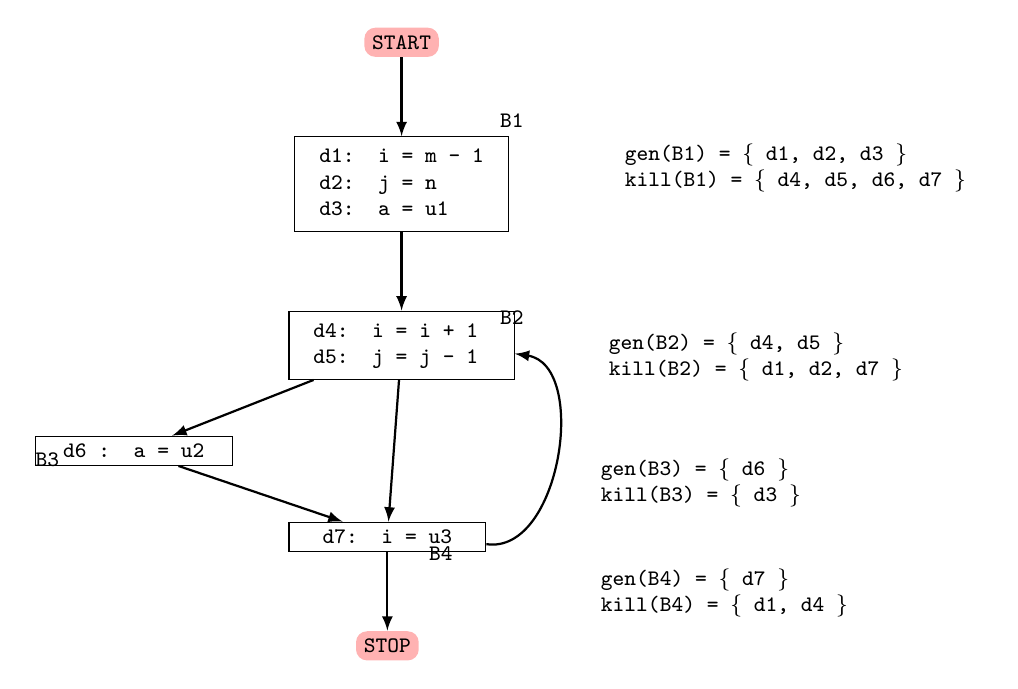
\begin{tikzpicture}[node distance=1cm,
        startstop/.style={rectangle,rounded corners,text centered,fill=red!30},
        process/.style={rectangle, minimum width=2.5cm, draw=black},
        arr/.style={thick,-latex}
        ]
        \footnotesize
        \node (in) [startstop] {\texttt{START}};
        \node (b1) [process,below=of in] 
            {\begin{tabular}{l} \texttt{d1: i = m - 1} \\ \texttt{d2: j = n} \\ \texttt{d3: a = u1} \end{tabular}};
        \draw[arr] (in) -- (b1);
        \node at (1.4,-1) {\texttt{B1}};
        \node at (5, -1.6) {\begin{tabular}{l} \texttt{gen(B1) = \{ d1, d2, d3 \}} \\ \texttt{kill(B1) = \{ d4, d5, d6, d7 \}} \end{tabular}};
        \node (b2) [process,below=of b1]
            {\begin{tabular}{l} \texttt{d4: i = i + 1} \\ \texttt{d5: j = j - 1 } \end{tabular}};
        \draw[arr] (b1) -- (b2);
        \node at (1.4,-3.5) {\texttt{B2}};
        \node at (4.5, -4) {\begin{tabular}{l} \texttt{gen(B2) = \{ d4, d5 \}} \\ \texttt{kill(B2) = \{ d1, d2, d7 \}}\end{tabular}};
        \node (b3) [process, below left=of b2] {\texttt{d6 : a = u2}};
        \draw[arr] (b2) -- (b3);
        \node at (-4.5,-5.3) {\texttt{B3}};
        \node at (3.8, -5.6) {\begin{tabular}{l} \texttt{gen(B3) = \{ d6 \}} \\ \texttt{kill(B3) = \{ d3 \}} \end{tabular}};
        \node (b4) [process, below right=of b3] {\texttt{d7: i = u3}};
        \draw[arr] (b3) -- (b4);
        \draw[arr] (b2) -- (b4);
        \draw[arr,bend right=90] (b4) to (b2);
        \node at (0.5,-6.5) {\texttt{B4}};
    \node at (4.1, -7) {\begin{tabular}{l} \texttt{gen(B4) = \{ d7 \}} \\ \texttt{kill(B4) = \{ d1, d4 \}} \end{tabular}};
        \node (out) [startstop, below=of b4] {\texttt{STOP}};
        \draw [arr] (b4) -- (out);
    \end{tikzpicture}
    \caption{Exemplu pentru definiții accesibile}
    \label{fig:rdef-ex1}
\end{figure}

Să studiem definițiile din blocul \texttt{B2}. Toate definițiile din blocul
\texttt{B1} ajung la începutul blocului \texttt{B2}. Definiția
\texttt{d5:\!\!\!\! j = j - 1} din blocul \texttt{B2} ajunge și la începutul blocului
\texttt{B2}, deoarece nu mai există altă definiție a lui \texttt{j} care să
se găsească în bucla ce duce înapoi în \texttt{B2}. Această definiție, însă,
distruge definiția \texttt{d2:\!\!\!\! j = n}, ceea ce o face să nu ajungă la
\texttt{B3} sau \texttt{B4}.

Pe de altă parte, instrucțiunea \texttt{d4:\!\!\!\! i = i + 1} din blocul \texttt{B2}
nu ajunge la începutul lui \texttt{B2}, deoarece variabila \texttt{i} este
mereu redefinită de \texttt{d7:\!\!\!\! i = u3}.

În fine, definiția \texttt{d6:\!\!\!\! a = u2} ajunge și ea la începutul blocului
\texttt{B2}.

\begin{remark}\label{rk:safe}
    Prin definirea definițiilor accesibile așa cum am făcut-o, pot exista
    in\-ad\-ver\-ten\-țe, însă toate sînt în direcția \emph{conservativă}, adică mai curînd
    se consideră aspecte redundante, decît să se omită unele. De exemplu, în codul:
    \begin{center}
        \begin{BVerbatim}
            if (a == b) { instrucțiune1 } 
            else if (a == b) { instrucțiune2 }
        \end{BVerbatim}
    \end{center}
    \texttt{instrucțiune2} nu se va atinge niciodată, pentru nicio valoare a lui \texttt{a}.

    Însă în general, problema dacă toate drumurile dintr-un graf de flux al datelor
    sînt parcurse este indecidabilă, astfel că alegem asumpția că ele sînt efectiv
    parcurse, chiar dacă acest lucru poate conduce la situații precum cea de mai
    sus. Eroarea în acest caz este de partea pozitivă, astfel că nu pierdem informație,
    ci cel mult avem o cantitate redundantă.
\end{remark}

%%%%%%%%%%%%%%%%%%%%%%%%%%%%%%%%%%%%%%%%%%%%%%%%%%%%%%%%%%%%%%%%%%%%%%
\section{Ecuații de transfer}

Arătăm acum modul în care se pot formula constrîngerile pentru problema
definițiilor accesibile. Începem prin studiul unei singure instrucțiuni:
\[
    \texttt{d: u = v + w}.
\]

Instrucțiunea generează o definiție \texttt{d} a unei variabile \texttt{u}
și distruge toate celelalte definiții din program care se adresează
variabilei \texttt{u}, dar nu afectează nicio altă definiție. Așadar,
funcția de transfer pentru definiția \texttt{d} poate fi scrisă:
\begin{equation}
    \label{eq:gen-kill}
    f_d(x) = \texttt{gen(d)} \cup (x - \texttt{kill(d)}),
\end{equation}
unde \texttt{gen(d) = \{d\}}, este mulțimea definițiilor
generate de instrucțiune, iar $ \texttt{kill(d)} $ este mulțimea
celorlalte definiții ale lui \texttt{u} din program.

În general funcția de transfer a unui bloc poate fi aflată prin
compunerea tuturor funcțiilor de transfer ale instrucțiunilor din interiorul
blocului. Se poate vedea ușor că prin compunerea a două funcții precum
cea de mai sus (ecuația~\eqref{eq:gen-kill}, pe care o vom numi ecuație
\texttt{gen-kill}) se obține tot o funcție cu aceeași formă.
\index{ecuație!\texttt{gen-kill}}

În general, avem:
\begin{equation}
    \label{eq:fb}
    f_b(x) = \texttt{gen(B)} \cup (x - \texttt{kill(B)},
\end{equation}
unde am notat:
\[
    \texttt{kill(B)} = \texttt{kill(1)} \cup \texttt{kill(2)} \cup \dots \cup \texttt{kill(n)},
\]
iar pentru generare, avem:
\begin{align*}
    \texttt{gen(B)} &= \texttt{gen(n)} \cup (\texttt{gen(n-1)} - \texttt{kill(n)}) \cup %
    (\texttt{gen(n-2)} - \texttt{kill(n-1)} - \texttt{kill(n)} \cup \\
                    & \dots \cup (\texttt{gen(1)} - \texttt{kill(2)} - \texttt{kill(3)} - %
                    \dots - \texttt{kill(n)})
\end{align*}

\index{definiții!expuse mai jos}
Mulțimea \texttt{gen} care rezultă dintr-un bloc se va numi mulțimea definițiilor
\emph{expuse mai jos}, deoarece această mulțime va conține toate definițiile
din bloc care sînt vizibile și imediat după bloc. Rezultă că o definiție dintr-un
bloc este expusă mai jos dacă și numai dacă nu este distrusă de o definiție a
aceleiași variabile în interiorul aceluiași bloc.

De cealaltă parte, mulțimea \texttt{kill} a unui bloc este pur și simplu reuniunea
tuturor definițiilor distruse de instrucțiuni individuale.

Remarcăm că, în general, o definiție poate apărea atît în mulțimea \texttt{gen},
cît și în \texttt{kill} ale unui bloc. Dacă acesta este cazul, atunci
considerăm că ea este generată, deoarece presupunem că mulțimea \texttt{kill}
acționează după mulțimea \texttt{gen}.

\begin{example}\label{exm:gen-kill}
    Considerăm blocul simplu \texttt{B}:
    \begin{align*}
        \texttt{d1:} \quad & \texttt{a = 3} \\
        \texttt{d2:} \quad & \texttt{a = 4}
    \end{align*}
    În acest caz, \texttt{gen(B) = \{d2\}}, deoarece \texttt{d1} nu este expusă
    mai jos. De asemenea, tot pentru acest bloc \texttt{kill(B) = \{d1, d2\}}, deoarece \texttt{d1}
    distruge \texttt{d2} și reciproc. Totuși, din cauza presupunerii de precedență,
    rezultatul funcției de transfer pentru acest bloc va include mereu \texttt{d2}.
\end{example}

%%%%%%%%%%%%%%%%%%%%%%%%%%%%%%%%%%%%%%%%%%%%%%%%%%%%%%%%%%%%%%%%%%%%%%

\section{Ecuațiile fluxului de control}

Considerăm acum constrîngerile care rezultă din fluxul de control dintre
blocurile de bază. Cum o definiție atinge un punct al programului dacă și numai
dacă există cel puțin un drum prin care definiția să se propage, avem:
\[
    \texttt{OUT[P]} \seq \texttt{IN[B]},
\]
unde \texttt{P} este un punct astfel încît să existe un drum de flux al
controlului pînă la blocul \texttt{B}. Însă, cum o definiție nu poate ajunge la
un punct decît dacă o face pe un drum, rezultă că \texttt{IN[B]} nu
depășește reuniunea definițiilor accesibile din toate blocurile ce-l
precedă pe \texttt{B}. Deci putem presupune că, în general, avem:
\[
    \texttt{IN[B]} = \bigcup_{\texttt{P} \downarrow \texttt{B}} \texttt{OUT[P]},
\]
unde am notat cu $ \texttt{P} \downarrow \texttt{B} $ faptul că punctul \texttt{P}
precede blocul \texttt{B}.

Putem privi această reuniune ca pe un operator \emph{meet} pentru
definițiile accesibile, ca în cazul laticelor.
\index{definiții!accesibile!meet}

%%%%%%%%%%%%%%%%%%%%%%%%%%%%%%%%%%%%%%%%%%%%%%%%%%%%%%%%%%%%%%%%%%%%%%
\section{Algoritm iterativ pentru definiții accesibile}
\index{definiții!accesibile!algoritm}

Vom presupune, ca o convenție de organizare, că orice graf de flux al
controlului are două blocuri goale: unul care reprezintă nodul de intrare
în graf (\texttt{ENTRY}), iar celălalt, de ieșire (\texttt{EXIT}), care reprezintă
punctul prin care trec toate căile de ieșire din graf.

Nicio definiție nu poate ajunge la nodul de intrare, deci funcția
de transfer pentru acest nod este funcția vidă:
\[
    \texttt{OUT[ENTRY]} = \emptyset.
\]

Pentru toate celelalte blocuri \texttt{B}, în afară de \texttt{ENTRY},
ecuațiile pe care vrem să le rezolvăm sînt:
\begin{align*}
    \texttt{OUT[B]} &= \texttt{gen(B)} \cup (\texttt{IN[B]} - \texttt{kill(B)}) \\
    \texttt{IN[B]} &= \bigcup_{\texttt{P} \downarrow \texttt{B}} \texttt{OUT[P]}.
\end{align*}

Algoritmul pe care îl prezentăm rezolvă exact acest sistem de ecuații.
Soluția sistemului va fi \emph{cel mai mic punct fix al ecuațiilor}, adică
acea soluție care asociază \texttt{IN} și \texttt{OUT} valorile ce se vor
regăsi în orice altă soluție. Mai mult, rezultatul algoritmului
este acceptabil, deoarece orice definiție pentru \texttt{IN} și \texttt{OUT}
va ajunge la punctul descris. Este, totodată, și o soluție dorită,
deoarece nu include nicio definiție care sigur nu este accesibilă.

Planul algoritmului este următorul:
\begin{itemize}
    \item \emph{Date de intrare:} Un graf de flux pentru care s-au calculat
        \texttt{kill(B)} și \texttt{gen(B)}, asociate tuturor blocurilor \texttt{B};
    \item \emph{Date de ieșire:} \texttt{IN[B]} și \texttt{OUT[B]}, adică
        mulțimile de definiții care ajung la punctele de intrare, respectiv de ieșire
        ale fiecărui bloc \texttt{B} din graful fluxului;
    \item \emph{Metoda:} Vom folosi o abordare iterativă, în care începem
        cu valoarea inițială $ \texttt{OUT[B]} = \emptyset $, pentru orice bloc \texttt{B}
        și vom ajunge prin convergență la valorile căutate pentru \texttt{IN} și \texttt{OUT}.
        În principiu, putem folosi o variabilă booleană care să ne arate dacă valorile
        pentru \texttt{IN} și \texttt{OUT} s-au schimbat la iterația curentă și să ne
        oprim atunci cînd nu se mai fac schimbări (i.e.\ avem convergență), dar vom
        presupune că mecanismele de modificare sînt subînțelese, deci putem afla
        și direct dacă s-au făcut sau nu modificări.

        Vom face referire la Algoritmul \ref{alg:rdef}, a cărui desfășurare urmează
        întocmai elementele de teorie prezentate pînă acum.
\end{itemize}

\begin{algorithm}
    \caption{Algoritm iterativ pentru definiții accesibile}
    \begin{algorithmic}[1]
        \Procedure{RDEF}{B}
            \State $ \texttt{OUT[ENTRY]} = \emptyset $
            \For{($\texttt{B} \neq \texttt{ENTRY}$)}
                \State $ \texttt{OUT[B]} = \emptyset $
            \EndFor
            \While{(\texttt{OUT} se schimbă)}
                \For{($\texttt{B} \neq \texttt{ENTRY}$)}
                    \State $ \texttt{IN[B]} = \bigcup_{\texttt{P} \downarrow \texttt{B}} \texttt{OUT[P]} $
                    \State $ \texttt{OUT[B]} = \texttt{gen(B)} \cup (\texttt{IN[B]} - \texttt{kill(B)}) $
                \EndFor
            \EndWhile
        \EndProcedure
    \end{algorithmic}
    \label{alg:rdef}
\end{algorithm}


Intuitiv, algoritmul propagă definițiile cît de departe pot ajunge fără a fi
distruse și prin aceasta, simulează toate execuțiile posibile ale programului.
Remarcăm că algoritmul se va opri, întrucît pentru orice bloc \texttt{B},
mulțimea \texttt{OUT[B]} nu se poate micșora --- atunci cînd este adăugată
o definiție, ea rămîne acolo. Deci în final, această mulțime va conține
cel mult toate definițiile din program, iar cînd nu se mai adaugă niciuna
la \texttt{OUT[B]}, programul se oprește. Totodată, această condiție de
oprire este una bună, deoarece dacă \texttt{OUT[B]} nu s-a schimbat,
atunci nu se va schimba nici \texttt{IN[B]} la iterația următoare,
ceea ce va face să nu se schimbe \texttt{OUT[B]} nici la iterația care
va urma, deci nu se mai schimbă nimic.

Numărul nodurilor din graful de flux este o margine superioară pentru numărul
de repetări ale buclei \textbf{while}. Aceasta se poate vedea prin faptul
că, dacă o definiție ajunge la un punct, nu o poate face decît pe o cale
care nu conține cicluri, iar numărul total de noduri din graf este o margine
superioară pentru nodurile din afara ciclurilor. Totodată, la fiecare
repetare a buclei \textbf{while}, definițiile se propagă cu cel puțin un
nod.

În ciuda aparențelor, algoritmul de mai sus poate fi făcut foarte eficient
folosind, de exemplu, \emph{vectori de biți} care să țină evidența
definițiilor active. Astfel, se consideră un vector de biți cu lungimea
egală cu numărul definițiilor din program, inițializat cu valoarea nulă
pe toate pozițiile, iar poziția \texttt{i} din vector devine \texttt{1}
atunci cînd definiția \texttt{di} este vizibilă la iterația curentă
prin program. Avantajul acestei abordări este că, de îndată ce am construit
vectorii de biți, manipularea lor se poate face foarte simplu, folosind
operații logice la nivel de biți. Un exemplu analizat este 
\cite[Example 9.12, p.~607]{aho}, alte detalii la \cite[\S 8.1]{much}, 
iar un algoritm implementat în C++ este 
\href{https://github.com/bhumbers/optcomp/blob/master/asst2/ClassicalDataflow/reaching-definitions.cpp}{aici}.

%%%%%%%%%%%%%%%%%%%%%%%%%%%%%%%%%%%%%%%%%%%%%%%%%%%%%%%%%%%%%%%%%%%%%%
\section{Exemplu suplimentar}

Preluăm acum un alt exemplu, din \cite{epfl}, pentru a ilustra și cazul
variabilelor ne\-i\-ni\-ți\-a\-li\-za\-te.

Notăm cu $ o_i = \{ (v_j, d_k) \} $ mulțimea de ieșire corespunzătoare
nodului $ i $ dintr-un graf de flux al controlului, care este o mulțime
de perechi alcătuite din variabile $ v_j $ definite la nodul $ k $
al grafului. De exemplu, $ o_5 = \{ (x, 3) \} $ va însemna că la ieșirea
din nodul al cincilea al grafului s-a propagat definiția variabilei $ x $,
definiție apărută la nodul al treilea. Alternativ, vom folosi și o scriere
de forma \texttt{o5 = {(x,3)}}, iar prin abuz de notație, \texttt{o5 - x}
va însemna, de exemplu, mulțimea definiților accesibile la ieșirea din
nodul 5, mai puțin toate definițiile lui \texttt{x}. Notația \texttt{o1 + o2}
va însemna reuniunea mulțimilor respective.

Așadar, avem figura \ref{fig:def-epfl}.

\begin{figure}[!htbp]
    \centering
    \usetikzlibrary{positioning}
    \usetikzlibrary{shapes.geometric}
    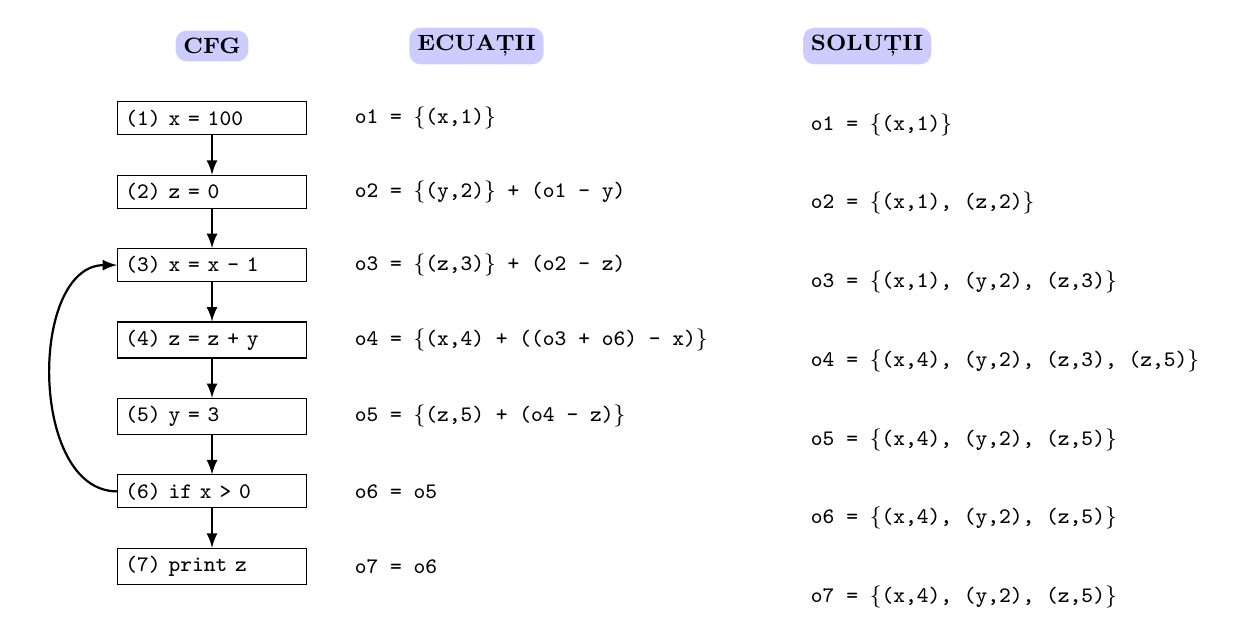
\begin{tikzpicture}[node distance=0.5cm,
        startstop/.style={rectangle,rounded corners,text centered,fill=blue!20},
        process/.style={rectangle, text width=2.2cm, draw=black},
        arr/.style={thick,-latex}
        ]
        \footnotesize
        \node (cfg) [startstop] at (0,0)              { \textbf{CFG} };
        \node (eq)  [startstop,right=of cfg] at (2,0) { \textbf{ECUAȚII} };
        \node (sol) [startstop, right=of eq] at (7,0) { \textbf{SOLUȚII} };
        \node (1) [process, below=of cfg] {\texttt{(1) x = 100}};
        \node (2) [process, below=of 1] {\texttt{(2) z = 0}};
        \node (3) [process, below=of 2] {\texttt{(3) x = x - 1}};
        \node (4) [process, below=of 3] {\texttt{(4) z = z + y}};
        \node (5) [process, below=of 4] {\texttt{(5) y = 3}};
        \node (6) [process, below=of 5] {\texttt{(6) if x > 0}};
        \node (7) [process, below=of 6] {\texttt{(7) print z}};
        \draw[arr] (1) -- (2) ;
        \draw[arr] (2) -- (3) ;
        \draw[arr] (3) -- (4) ;
        \draw[arr] (4) -- (5) ;
        \draw[arr] (5) -- (6) ;
        \draw[arr] (6) -- (7);
        \draw[arr,bend left=90] (6) to (3);
        \node (e1) [right=of 1] {\texttt{o1 = \{(x,1)\}}};
        \node (e2) [right=of 2] {\texttt{o2 = \{(y,2)\} + (o1 - y)}};
        \node (e3) [right=of 3] {\texttt{o3 = \{(z,3)\} + (o2 - z)}};
        \node (e4) [right=of 4] {\texttt{o4 = \{(x,4) + ((o3 + o6) - x)\}}};
        \node (e5) [right=of 5] {\texttt{o5 = \{(z,5) + (o4 - z)\}}};
        \node (e6) [right=of 6] {\texttt{o6 = o5}};
        \node (e7) [right=of 7] {\texttt{o7 = o6}};
        \node (s1) [right=of e1] at (7,-1) {\texttt{o1 = \{(x,1)\}}};
        \node (s2) [right=of e2] at (7,-2) {\texttt{o2 = \{(x,1), (z,2)\}}};
        \node (s3) [right=of e3] at (7,-3) {\texttt{o3 = \{(x,1), (y,2), (z,3)\}}};
        \node (s4) [right=of e4] at (7,-4) {\texttt{o4 = \{(x,4), (y,2), (z,3), (z,5)\}}};
        \node (s5) [right=of e5] at (7,-5) {\texttt{o5 = \{(x,4), (y,2), (z,5)\}}};
        \node (s6) [right=of e6] at (7,-6) {\texttt{o6 = \{(x,4), (y,2), (z,5)\}}};
        \node (s7) [right=of e6] at (7,-7) {\texttt{o7 = \{(x,4), (y,2), (z,5)\}}};
    \end{tikzpicture}
    \caption{Exemplu pentru definiții accesibile}
    \label{fig:def-epfl}
\end{figure}


Concluzia analizei este că o singură definiție a lui \texttt{y} ajunge la nodul final,
anume definiția din nodul 2, \texttt{y = 3}. Rezultă că pentru optimizare, se poate
înlocui în nodul 5 \texttt{z = z + 3}, valoarea accesibilă a lui \texttt{y}.

Cazul variabilelor neinițializate poate fi tratat cu o analiză similară.
Să considerăm acum situația în care se omite definiția \texttt{y = 3} în nodul 2,
ca în figura \ref{fig:y-neinit}.

\begin{figure}[!htbp]
    \centering
    \usetikzlibrary{positioning}
    \usetikzlibrary{shapes.geometric}
    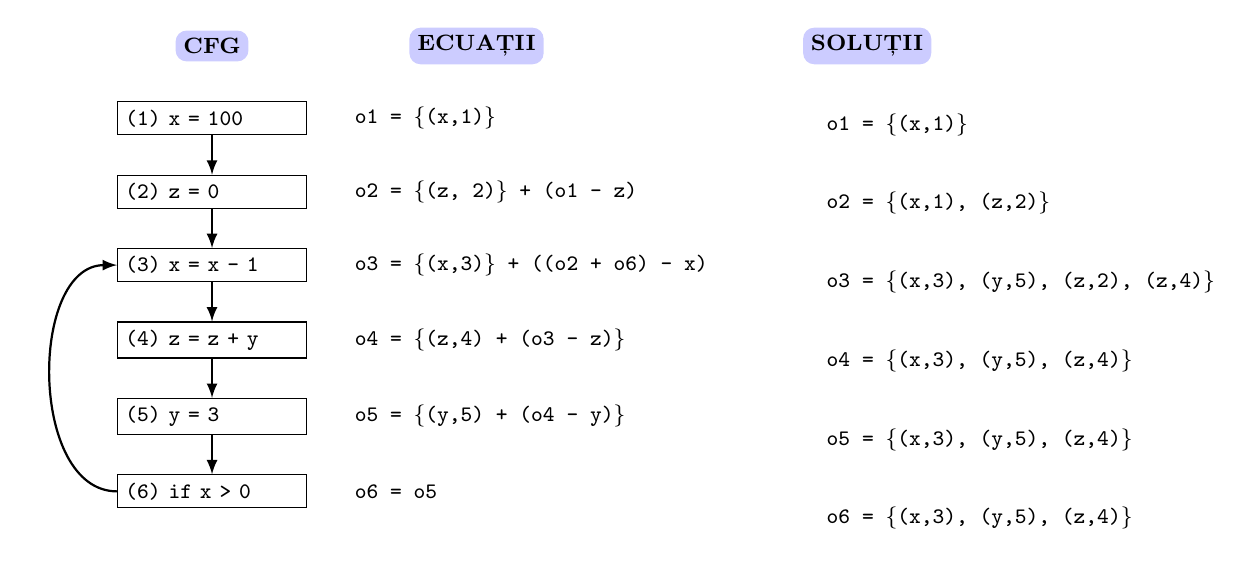
\begin{tikzpicture}[node distance=0.5cm,
        startstop/.style={rectangle,rounded corners,text centered,fill=blue!20},
        process/.style={rectangle, text width=2.2cm, draw=black},
        arr/.style={thick,-latex}
        ]
        \footnotesize
        \node (cfg) [startstop] at (0,0)              { \textbf{CFG} };
        \node (eq)  [startstop,right=of cfg] at (2,0) { \textbf{ECUAȚII} };
        \node (sol) [startstop, right=of eq] at (7,0) { \textbf{SOLUȚII} };
        \node (1) [process, below=of cfg] {\texttt{(1) x = 100}};
        \node (2) [process, below=of 1] {\texttt{(2) z = 0}};
        \node (3) [process, below=of 2] {\texttt{(3) x = x - 1}};
        \node (4) [process, below=of 3] {\texttt{(4) z = z + y}};
        \node (5) [process, below=of 4] {\texttt{(5) y = 3}};
        \node (6) [process, below=of 5] {\texttt{(6) if x > 0}};
        \draw[arr] (1) -- (2) ;
        \draw[arr] (2) -- (3) ;
        \draw[arr] (3) -- (4) ;
        \draw[arr] (4) -- (5) ;
        \draw[arr] (5) -- (6) ;
        \draw[arr,bend left=90] (6) to (3);
        \node (e1) [right=of 1] {\texttt{o1 = \{(x,1)\}}};
        \node (e2) [right=of 2] {\texttt{o2 = \{(z, 2)\} + (o1 - z)}};
        \node (e3) [right=of 3] {\texttt{o3 = \{(x,3)\} + ((o2 + o6) - x)}};
        \node (e4) [right=of 4] {\texttt{o4 = \{(z,4) + (o3 - z)\}}};
        \node (e5) [right=of 5] {\texttt{o5 = \{(y,5) + (o4 - y)\}}};
        \node (e6) [right=of 6] {\texttt{o6 = o5}};
        \node (s1) [right=of e1] at (7.2,-1) {\texttt{o1 = \{(x,1)\}}};
        \node (s2) [right=of e2] at (7.2,-2) {\texttt{o2 = \{(x,1), (z,2)\}}};
        \node (s3) [right=of e3] at (7.2,-3) {\texttt{o3 = \{(x,3), (y,5), (z,2), (z,4)\}}};
        \node (s4) [right=of e4] at (7.2,-4) {\texttt{o4 = \{(x,3), (y,5), (z,4)\}}};
        \node (s5) [right=of e5] at (7.2,-5) {\texttt{o5 = \{(x,3), (y,5), (z,4)\}}};
        \node (s6) [right=of e6] at (7.2,-6) {\texttt{o6 = \{(x,3), (y,5), (z,4)\}}};
    \end{tikzpicture}
    \caption{Exemplu pentru variabilă neinițializată \texttt{y}}
    \label{fig:y-neinit}
\end{figure}


Conform analizei, am putea crede că \texttt{y} poate fi înlocuită cu valoarea
din definiția 5 chiar și în nodul 4, ceea ce este evident fals!

Soluția problemei este să se înceapă analiza cu toate variabilele inițializate.
Cele care sînt inițializate efectiv sînt înregistrate în nodul corespunzător,
iar cele neinițializate încă sînt înregistrate ca și cum ar fi fost inițializate
într-un punct oarecare. Astfel, am obține în exemplul din figura \ref{fig:y-neinit}:
\begin{center}
    \begin{BVerbatim}
        o1 = {(x,1), (y,?), (z,?)}
    \end{BVerbatim}
\end{center}
și constatăm că \qq{definiția} \texttt{(y,?)} se propagă pînă în \texttt{o4},
inclusiv. Așadar, nu se poate înlocui \texttt{y} cu \texttt{3} mai devreme.


%%% Local Variables:
%%% mode: latex
%%% TeX-master: "../static"
%%% End:

